\section{Liegengebliebener Schnee}
\label{sec:fallen_snow}

\subsection{Einleitung}

In diesem Abschnitt wird die Erzeugung der Schneedecke
besprochen. Diese stellt eine Erweiterung der Kollisionscodes für die
Schneeflocken dar. Statt nur die Position der Flocke neu zu setzen,
wird der Punkt des Auftreffens weiter verarbeitet.

Für die Schneedecke wurden wurden insgesamt zwei Ansätze
umgesetzt. Zuerst ein auf Texturen basierender, der allerdings keine
Schneegeometrie erlaubt -- also Schneehügel, die sich auftürmen.

Wegen gravierender Nachteile dieses Verfahrens wurde danach ein
anderer Ansatz verfolgt, der mit Hilfe des Marching Cubes-Algorithmus
ein \emph{Mesh} für den Schnee erzeugt. Dieses Verfahren wurde zuerst
auf der GPU und später auf der CPU implementiert. Es sollen die
Unterschiede in den Implementierungen herausgestellt werden.

\subsection{Schneedecke mit Texturen}

Die moderne Computergrafik nutzt für die realistische Einfärbung von
Oberflächen \PimiddyBegriff{Texture Mapping}, also das Projizieren
eines Bildes auf die einzufärbende Oberfläche. Heutige Grafikkarten
unterstützen auch \PimiddyBegriff{Multitexturing}, um mehrere
Texturebenen gleichzeitig auf eine Oberfläche abzubilden. Der erste
Ansatz, eine Schneedecke zu visualisieren bestand darin, sie als
zusätzliche Textur auf den Oberflächen zu modellieren, welche anfangs
komplett durchsichtig ist und mit der Zeit eine weißliche Färbung
annimmt, wenn Flocken auf der Oberfläche auftreffen.

Es ist aus OpenCL heraus möglich, in (zweidimensionale) Texturen zu
schreiben. Daher kann man im Kernel, der die Bewegung der
Schneeflocken durchführt, folgendes Verfahren für die Generierung
einer Schneedecke umsetzen (\Pimiddyvgl
\autoref{fig:implementation_fallen_snow_textures_principle}):

\begin{enumerate}
\item Reserviere für jede Oberfläche jedes Objekts neben der
Farbtextur eine zweite Textur für die Schneedecke. Diese Texturen sollten
anfangs komplett durchsichtig sein.
\item Beim Auftreffen einer Schneeflocke auf ein Hindernis, bestimme
das getroffene Objekt und die Oberfläche auf dem Objekt, die getroffen
wurde. Bestimme daraus die Textur, die zu der Oberfläche gehört.
\item Durch einen Koordinatensystemwechsel, bestimme den Pixel auf der
Textur, der von der Flocke getroffen wurde.
\item Erhöhe den Wert des Pixels um einen vorher gewählten Wert, um es
ein wenig weißer und untransparenter zu machen.
\item Vermische beim Rendern die Oberflächentextur und die
Schneetextur, sodass die Schneedecke sichtbar wird.
\end{enumerate}

\begin{figure}[h]
\centering
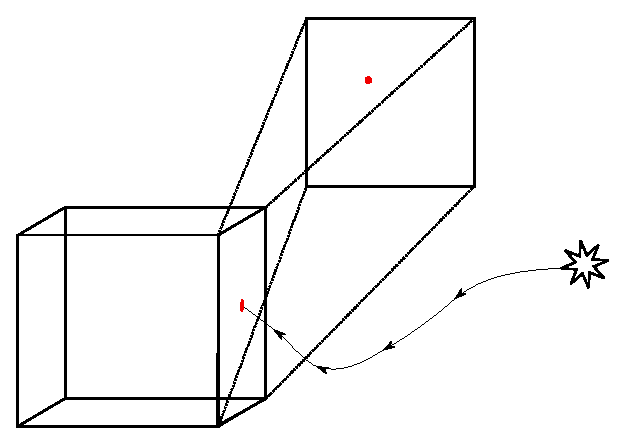
\includegraphics[width=12cm]{images/snow_cover_textures_principle}
\caption{Das Funktionsprinzip des Algorithmus für die Texturschneedecke verdeutlicht.}
\label{fig:implementation_fallen_snow_textures_principle}
\end{figure}

Der Ansatz liefert relativ gute Ergebnisse, es ergeben sich aber
signifikante Hürden:

\begin{enumerate}
\item Es können keine Schneehügel umgesetzt werden, die sich
auftürmen, da die Geometrie nicht verändert wird, nur die
Oberflächeneigenschaften.
\item Es muss wesentlich mehr Speicherplatz aufgewendet werden, um für
jede Oberfläche eine zweite Textur zu reservieren. Zudem ist unklar,
wie groß die Schneetextur sein sollte. Bei kleineren
Flächen bietet sich auch eine kleinere Textur an, aber eine Normierung
zu finden, ist ein schwierigeres Problem. Um Platz zu sparen, könnte
man die Textur zu einer Oberfläche auch erst erzeugen, wenn wirklich
Schnee auf ihr aufgetroffen ist.
\item Die zu einem Auftreffpunkt gehörige Textur in angemessener Zeit
zu bestimmen, benötigt eine Struktur, die den Raum effizient aufteilt.
\item Stabilitätseigenschaften wie die Bildung von Schneelawinen sind
nicht einfach zu integrieren.
\end{enumerate}

\begin{figure}[h]
\centering
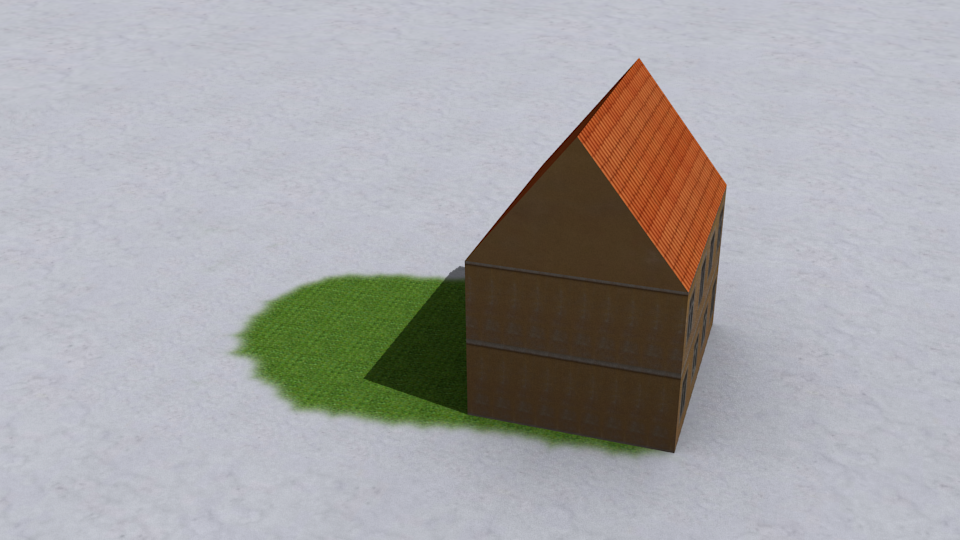
\includegraphics[width=14cm]{images/snow_cover_textures}
\caption{Die Schneedecke mit Texturen. Nur der Boden verwendet das Verfahren.}
\label{fig:implementation_fallen_snow_textures}
\end{figure}

Aufgrund dieser Nachteile wurde lediglich eine Form des Verfahrens
umgesetzt, die für den Boden der Simulation eine Schneedecke
erzeugt. \autoref{fig:implementation_fallen_snow_textures} zeigt das
Ergebnis.

\subsection{Schneedecke als Mesh}

\subsubsection{Einleitung}

Statt die Schneedecke als reine Oberflächeneigenschaft zu modellieren,
wird jetzt ein Ansatz vorgestellt, der die \emph{Schneedichte} an
jedem Punkt im Raum betrachtet. Diese Dichte wird mit Hilfe des
Marching Cubes-Algorithmus (MC) in ein Mesh verwandelt, welches dann
texturiert und beleuchtet wird.

Auf diese Weise können auch Schneehügel entstehen und
Stabilitätsbedingungen lassen sich einfacher integrieren. Viele der
Nachteile des Texturansatzes werden mit diesem Vorgehen behoben. Aber
das Verfahren hat auch Nachteile, wie der hohe Rechen- und
Speicherbedarf.

Es wird zuerst besprochen, wie das Dichtefeld aufgebaut wird und was
der Marching Cubes-Algorithmus schließlich als Eingabe erhält. Danach
wird der Algorithmus selbst grob erklärt. Schließlich werden die zwei
umgesetzten Implementierungen für GPU und CPU verglichen und die
endgültige Integration in die Anwendung erläutert.

\subsubsection{Aufbau der Schneedichte}

Trifft eine Schneeflocke auf ein Hindernis, also einen Voxel mit
Boundarywert $1$, so wird sie auf eine neue, zufällige Position
zurückgesetzt. Dies ist der Zeitpunkt, an dem die abgelagerte
Schneemenge in einer entsprechenden Datenstruktur erhöht werden muss.

Man legt ein weiteres Skalarfeld \PimiddyInlineCode{snow\_density} an,
welches die Schneemenge in den Gitterzellen der Simulation enthält
(\PimiddyzB gemessen in Gramm). Beim Auftreffen einer Schneeflocke an
einem Voxel wird der Eintrag an dieser Stelle des Skalarfeldes um das
Gewicht der Schneeflocke erhöht. Mit dieser einfachen Herangehensweise
ergeben sich zwei Probleme:

\begin{enumerate}
\item Der Test auf Kollision geschieht ein Voxelschicht
\PimiddyQuotes{zu spät}. Testet man, ob die Schneeflocke \emph{in}
einem Hindernis ist und erhöht \emph{dort} die Schneemenge, steckt
auch der Schnee im Hindernis, nicht an seiner Oberfläche.
\item Es können sich ohne weitere Stabilitätsbedingungen keine
Schneehaufen oder dickere Schneedecken bilden, denn der Kollisionscode
für die Schneeflocke beachtet nur das Feld
\PimiddyInlineCode{boundary}, nicht die Schneedichte. Voxel, die keine
Hindernisvoxel sind, können keinen Schnee ansammeln.
\end{enumerate}

Zur Lösung diese Probleme wird ein weiteres Skalarfeld eingeführt, das
\PimiddyBegriff{Aktivitätsfeld} \PimiddyInlineCode{activity}. Dieses
Feld wird im Kollisionscode der Schneeflocken statt
\PimiddyInlineCode{boundary} verwendet. Es ist also ebenfalls ein
binäres Feld -- ein Voxel kann nur die Werte $0$ oder $1$ annehmen.

Das Aktivitätsfeld wird in jedem Simulationsdurchlauf abgeleitet aus
den Feldern \PimiddyInlineCode{boundary} und
\PimiddyInlineCode{snow\_density}. Es ist an einer Gitterzelle
$(x,y,z)$ genau dann $1$, wenn eine der folgenden Bedingungen
zutrifft:

\begin{enumerate}
\item Ein Nachbarfeld von $(x,y,z)$ im Feld
\PimiddyInlineCode{boundary} hat den Wert 1. Auf diese Weise wird das
erste oben besprochene Problem gelöst, denn die Flocken kollidieren so
eine \PimiddyQuotes{Schicht} vor dem Hindernis, und dort wird auch die
Schneedichte erhöht. Es spielt in diesem Fall keine besondere Rolle,
welche Nachbarschaft gewählt wird.
\item Die Schneedichte in \PimiddyInlineCode{snow\_density} ist größer
als ein bestimmter Schwellenwert. So wird das zweite Problem gelöst,
denn bereits gefallener Schnee wirkt sich jetzt auf den Kollisionscode
aus. Man könnte alternativ an dieser Stelle das Feld
\PimiddyInlineCode{boundary} auf $1$ setzen, damit sich Schneehaufen
sogar auf die Windsimulation auswirken.
\end{enumerate}

Als Eingabe für den Marching Cubes-Algorithmus dient allerdings
weiterhin das Feld \PimiddyInlineCode{snow\_density}, das die
Schneedichte enthält.

\subsubsection{Der Marching Cubes-Algorithmus}

Der Marching Cubes-Algorithmus wurde 1987 von
\PimiddyName{William E. Lorensen} und \PimiddyName{Harvey E. Cline}
als Ergebnis einer Forschungsarbeit für die Forschungsabteilung des
Unternehmens General Electric in der Zeitschrift Computer Graphics
vorgestellt\cite{Lorensen:1987:MCH:37402.37422}. Der Algorithmus stand
20 Jahre lang unter einem Patent, seit 2005 kann er frei verwendet
werden.

Ursprünglich war MC für bildgebende Verfahren in der Medizin
gedacht. Medizinische Geräte wie ein MRT-Scanner geben
dreidimensionale Punktwolken zurück, die dann entweder
\PimiddyQuotes{scheibenweise} als 2D-Bilder betrachtet werden können
oder als dreidimensionales Modell. Bei dem Modell handelt es sich
natürlich nur um eine Annäherung, die stark von der Qualität der
Punktwolke abhängt.

Als Eingabe erhält der Algorithmus in dieser Arbeit statt einer
Punktwolke ein regelmäßiges Gitter mit skalaren Werten -- \PimiddyzB
die Schneedichte --, sowie einen \PimiddyBegriff{Isowert}, der angibt,
ab wann eine Gitterzelle als \PimiddyQuotes{fest} angesehen wird.
Benachbarte, feste Zellen werden vom Algorithmus in ein
zusammenhängendes Mesh verwandelt.

Die Ausgabe des Algorithmus ist eine Liste von Dreiecken, deren
Eckpunkte zunächst nur durch ihre Position gegeben sind. Der
Algorithmus wird später um Normalen und Texturkoordinaten erweitert.

Das Eingabefeld wird zellenweise bearbeitet. Für jede Zelle $n_1$
werden die unmittelbaren Nachbarzellen $n_2,\ldots,n_8$ bestimmt,
genau wie das in \autoref{sec:implementation_wind_advection} geschehen
ist. Der Dichtewert an jeder Ecke des durch die $n_i$ beschriebnen
Würfels wird mit dem vorgegebenen Isowert verglichen. Es entsteht eine
1, wenn der Wert über dem Isowert liegt, ansonsten eine 0. Als Ausgabe
für eine Zelle erhält man auf diese Weise eine 8-Bit-Zahl und
$2^8=256$ mögliche Kombinationen von Werten für einen Würfel.

Die 8-Bit-Zahl wird als Index für eine Lookuptabelle verwendet, in der
die \emph{Dreiecke} stehen, die zu dieser Kombination von Isowerten
gehören (siehe
\autoref{fig:implementation_fallen_snow_marching_cubes_combinations}). Diese
Liste ist leer für den Fall, dass keiner der Werte über dem Isowert
liegt. Ansonsten werden die Dreiecke zur Ausgabe hinzugefügt und die
nächste Zelle wird betrachtet.

Wahlweise werden die Eckpunkte der Dreiecke in diesem letzten Schritt
leicht verschoben um der Tatsache gerecht zu werden, dass einige Werte
\Pimiddyggf weit über dem Isowert liegen und andere nur leicht
darüber.

Außerdem kann die Lookuptabelle aufgrund von Symmetrieeigenschaften
von 256 auf 15 Fälle reduziert werden.

\begin{figure}[h]
\centering
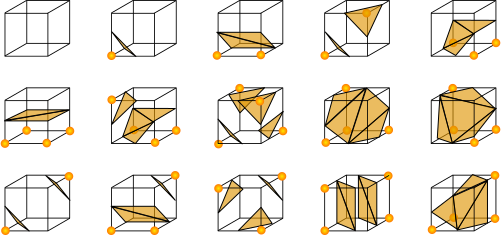
\includegraphics[width=12cm]{images/marching_cubes_combinations}
\caption{Die durch Symmetrieeigenschaften auf 15 Fälle reduzierte Lookuptabelle für die Dreiecke in einem Würfel}
\label{fig:implementation_fallen_snow_marching_cubes_combinations}
\end{figure}

\subsubsection{Normalen und Texturen}

\begin{figure}[h]
\centering
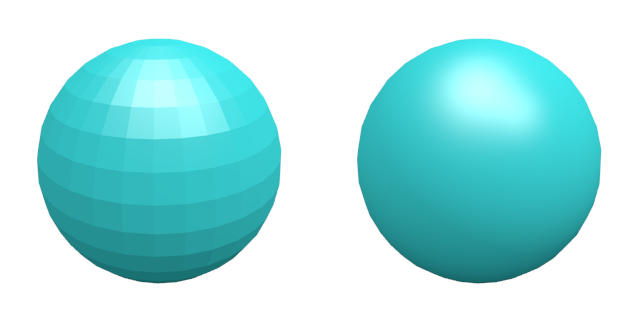
\includegraphics[width=10cm]{images/shading_comparison}
\caption{Vergleich zwischen Flat Shading (links), was durch Flächennormalen entsteht, und Smooth Shading (rechts)}
\label{fig:implementation_fallen_snow_shading_comparison}
\end{figure}

Der eben beschriebene Algorithmus gibt eine Liste von Dreiecken aus,
an deren Eckpunkten lediglich Informationen über die Position
enthalten sind. Diese Dreiecksmenge kann nicht ad hoc texturiert
werden, denn es fehlen Texturkoordinaten. Auch die Beleuchtung fällt
ohne Normaleninformationen schwer. In diesem Abschnitt werden Lösungen
für beide Probleme besprochen.

Um Normalen für das Mesh zu erhalten, gibt es mehrere
Möglichkeiten. Die einfachste besteht darin, für jedes Dreieck
$\vec{p}_1,\vec{p}_2,\vec{p}_3$ eine Flächennormale mit Hilfe des Kreuzprodukts zu bestimmen:
\begin{align}
\vec{n} = (\vec{p}_2 - \vec{p}_1) \times (\vec{p}_3 - \vec{p}_1)
\end{align}
Dies ist ohne Weiteres umsetzbar, es ermöglicht allerdings nur
\PimiddyBegriff{Flat Shading} als Beleuchtungsmodell, also keine
sanften Übergänge zwischen benachbarten Flächen (siehe
\autoref{fig:implementation_fallen_snow_shading_comparison}).

Um zwischen den Flächen interpolierte Normalen zu erhalten könnte man
für jeden Punkt jeder Fläche alle benachbarten Flächen suchen und
mitteln. Da die Dreiecksliste aus der MC-Ausgabe aber keine
hilfreichen topologischen Informationen enthält, benötigt dieses
Vorgehen quadratische Laufzeit.

Stattdessen benutzt man nicht die \emph{Ausgabe} des Algorithmus,
sondern das \emph{Eingabefeld}, um die Normalen zu berechnen. Es wird
der \emph{Gradient} des Eingabefeldes als Quelle für die Normalen
verwendet. Dies fällt besonders einfach aus, da der Code zum Berechnen
des Gradienten schon existiert -- er wird in
\autoref{sec:implementation_wind_projection} besprochen.

Um das Mesh zu texturieren wurden zwei Ansätze verfolgt, die beide
erläutert werden. Der erste basiert auf Noise aus 3D-Texturen und
benötigt keine weiteren Daten außer den Eckpunkten der Dreiecke. Der
zweite wird als \PimiddyBegriff{triplanare Texturierung} bezeichnet
und benötigt die Flächennormalen der Dreiecke. Die Technik wurde unter
anderem in \cite{Nguyen:2007:GG:1407436} vorgestellt und liefert
visuall ansprechende Ergebnisse.

Hat man nur die Positionen der Dreieckspunkte zur Verfügung und will
Farben bestimmen, sodass die Oberfläche der einer Schneedecke ähnelt,
liegt es nahe, die Farbdaten direkt aus einer dreidimensionalen Textur
zu laden. Diese 3D-Textur repräsentiert einen \PimiddyQuotes{Block}
aus Schnee, in den man mittels einer Koordinate hineingreifen kann und
die Schneefarbe innerhalb des Volumens erhält. Es stellt sich die
Frage, woher man diese Textur bekommt und wie groß sie sein muss.

\begin{figure}[h]
	\begin{subfigure}[t]{0.5\textwidth}
		\centering
		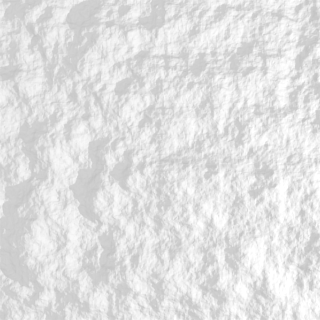
\includegraphics[width=\textwidth]{images/perlin_noise_snow}
		\caption{Eine mit Perlin-Noise generierte Schneedecke}
		\label{fig:implementation_fallen_snow_perlin_noise_snow}
	\end{subfigure}
	~
	\begin{subfigure}[t]{0.5\textwidth}
		\centering
		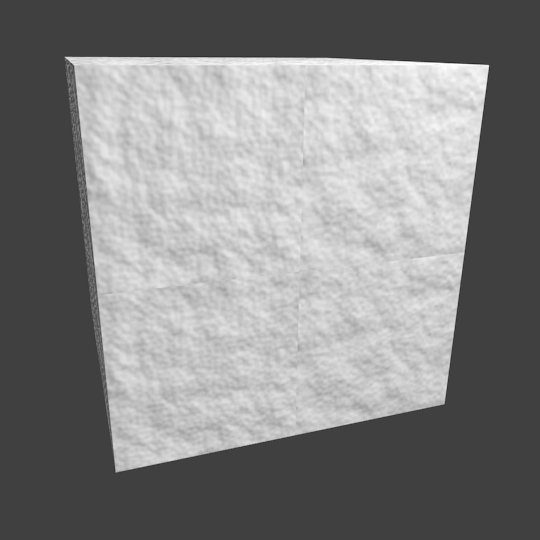
\includegraphics[width=\textwidth]{images/noise_texture_artifact}
		\caption{Artefakte, die bei einer nichtkachelbaren 3D-Texture auftreten}
		\label{fig:implementation_fallen_snow_perlin_noise_artifact}
	\end{subfigure}
        \caption{Generierung der Schneetextur aus Perlin-Noise}
\end{figure}

Die Größe der Textur ist davon abhängig, wie groß der
Simulationsbereich gewählt wird. Simuliert man einen 100 Meter großen
Bereich und möchte Details erkennen, die 10cm groß sind, benötigt man
bereits eine $1000 \times 1000 \times 1000$ große Textur, die bei 8
Bit Graustufen schon annähernd einen Gigabyte Platz
verbraucht. Heutige Grafikkarten haben allerdings \emph{insgesamt} nur
einen Gigabyte Videospeicher. Es ist daher sinnvoll, eine kleinere
Volumentextur zu verwenden, die aber an allen Seiten nahtlos
anschließt (\PimiddyBegriff{kachelbar} ist), sodass sie mehrfach auf
jeder Achse wiederholt werden kann. Es bleibt aber noch zu klären, wie
man so eine Textur herstellt.

Bei zweidimensionalen Texturen reicht es oft, Fotos der entsprechenden
Oberfläche zu machen und in eine Textur zu konvertieren. Bei
Volumendaten hingegen greift man häufig auf prozedurale Generierung
zurück, also der algorithmischen Erstellung von
Farbwerten. \autoref{fig:implementation_fallen_snow_perlin_noise_snow}
zeigt beispielsweise eine 2D-Textur für eine Schneedecke, die
algorithmisch mittels Perlin-Noise\cite{Perlin:2002:IN:566654.566636}
generiert wurde.

Die Generierung von dreidimensionalem Noise ist jedoch an sich schon
sehr aufwändig. Die Anforderung, dass die Textur kachelbar sein muss,
erhöht den Konstruktionsaufwand weiter immens. Der Ansatz wurde daher
nur mit nichtkachelbaren Texturen umgesetzt, was zu deutlichen
Bildfehlern führte (\Pimiddyvgl
\autoref{implementation_fallen_snow_perlin_noise_artifact}).

In der finalen Implementierung wurde stattdessen triplanare
Texturierung verwendet. Diese Methode ist im Vergleich sehr
platzsparend, dafür aber etwas rechenaufwändiger als eine
3D-Textur. Sie erlaubt es, steilen Oberflächen eine andere Textur zu
geben als annähernd waagerechten, was den Realismusgrad beträchtlich
erhöht. Das Verfahren lässt ich komplett in GLSL umsetzen und benötigt
keine weiteren Daten von außen.

Die Idee hinter dem Verfahren ist, dass man drei 2D-Texturen vorgibt,
jeweils für die $xy$-Ebene, die $xz$-Ebene und die $yz$-Ebene. Die
Normale an einem Dreieckspunkt entscheidet, welche Textur wie stark
zur Färbung des Dreiecks beiträgt. Ein horizontales Dreieck mit
Normale $(0,1,0)$ verwendet beispielsweise nur die zur $xz$-Ebene
gehörige Textur.

Für den Schnee wird später eine relativ glatte Textur auf der
$xz$-Ebene verwendet und zwei etwas \PimiddyQuotes{rauere} Texturen
für die beiden anderen Ebenen. Dadurch, dass man die Normalen an den
Eckpunkten interpoliert, kann man auch gekrümmte Flächen gut
einfärben, sofern sich die Texturen nicht zu stark unterscheiden. Die
folgende Funktion erhält die Oberflächennormale und berechnet daraus
die Gewichte für die drei Texturen. Sie werden als dreidimensionaler
Vektor zurückgegeben:

\begin{minted}[frame=lines]{glsl}
vec3
calculate_blend_weights(
    vec3 normal_vector)
{
    vec3 blend_weights =
            max(
                (abs(normal_vector) - 0.2) * 7.0,
                0.0);

    float blend_sum =
        blend_weights.x + blend_weights.y + blend_weights.z;

    // Achtung: Eventuell Division durch 0!
    if(blend_sum < 0.001)
        return vec3(1.0,0.0,0.0);

    blend_weights /=
        blend_sum;

    return
        blend_weights;
}
\end{minted}

Der Normalenvektor wird zunächst verschoben und gewichtet. Die Werte
$0.2$ und $7$ sind Erfahrungswerte, um das Überblenden zwischen den
Texturausrichtungen etwas schöner zu gestalten. Sie wurden direkt aus
\cite{Nguyen:2007:GG:1407436} übernommen. Danach wird der Vektor durch
die Summe seiner Komponenten geteilt, damit sich alle Komponenten zu 1
aufaddieren.

\begin{figure}[h]
\centering
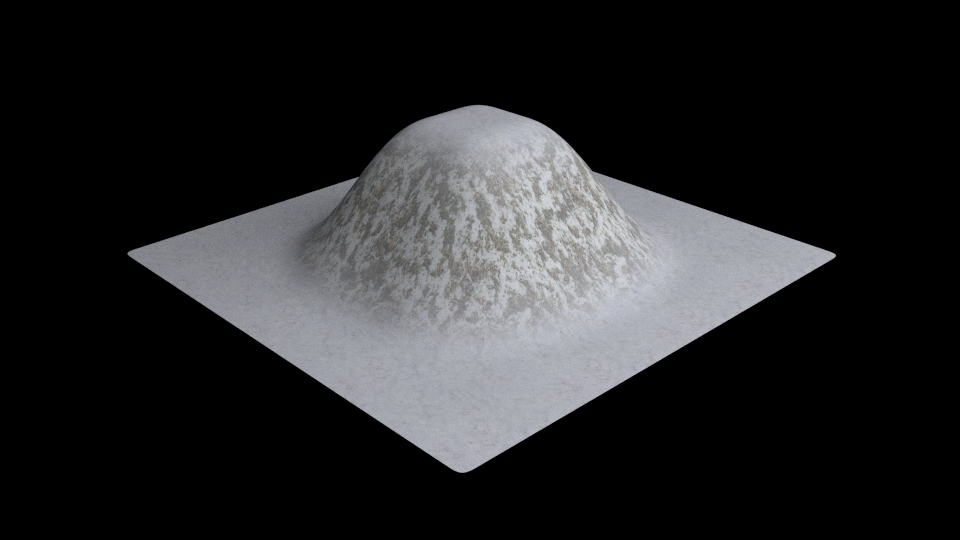
\includegraphics[width=12cm]{images/triplanar_mountain}
\caption{Die triplanare Texturierung einer Anhöhe mit zwei Texturen.}
\label{fig:implementation_fallen_snow_triplanar_mountain}
\end{figure}

Für jede der drei Texturen berechnen sich die Texturkoordinaten, indem
man aus der Position des Dreieckspunktes jeweils die beiden Achsen
nimmt, die die Ebene aufspannen. Die folgende Funktion erhält die
Position des Punktes in Weltkoordinaten, die grade errechneten
Gewichte und die Texturen und berechnet die endgültige Farbe:

\begin{minted}[frame=lines]{glsl}
vec4
calculate_blended_color(
    vec3 blend_weights,
    vec3 world_position,
    uniform sampler2D steep_texture,
    uniform sampler2D flat_texture)
{
    vec2 coord1 = world_position.yz,
         coord2 = world_position.zx,
         coord3 = world_position.xy;

    vec4 col1 = texture(steep_texture,coord1),
         col2 = texture(flat_texture,coord2),
         col3 = texture(steep_texture,coord3);

    return col1 * blend_weights.x +
           col2 * blend_weights.y +
           col3 * blend_weights.z;
}
\end{minted}

\subsubsection{Implementierungen}

In diesem Abschnitt werden die MC-Implementierungen auf der GPU und
der CPU besprochen. Dabei soll deutlich werden, was die jeweiligen
Vor- und Nachteile sind und wieso die endgültige Anwendung schließlich
die CPU-Implementierung einsetzt.

\subsubsection{GPU-Implementierung}

Der Marching Cubes-Algorithmus ist im Wesentlichen datenparallel. Jede
Zelle des Gitters kann unabhängig vom Rest bearbeitet werden. Daher
liegt es auch hier nahe, die GPU für die Konvertierung der Schneedecke
zu verwenden. Dies erweist sich jedoch in der Praxis als schwierig,
denn obwohl die Zellen an sich unabhängig zu bearbeiten sind, werden
für jede Zelle unterschiedlich viele Dreiecke erzeugt. Bei den bisher
behandelten datenparallelen Problemen war die Anzahl der Elemente der
Eingabe stets gleich der Anzahl der Elemente der Ausgabe. Hierbei
konnte sich die Größe der Eingabe- und Ausgabeelemente jedoch
unterscheiden (wie bei der Divergenz, wo ein Vektorfeld zu einem
Skalarfeld wurde). Der MC-Algorithmus passt nicht in dieses Schema.

In einer solchen Situation verwendet man üblicherweise eine
\PimiddyBegriff{Reduktion} (auch \PimiddyBegriff{Scan}
genannt\cite{Blelloch1989}). Reduktionen sind algorithmische
Grundbausteine auf parallelen Systemen. Mit ihnen können scheinbar nur
sequentiell (und damit schlecht) lösbare Operationen wie die
Summenbildung effizient parallel umgesetzt werden. Reduktionen sollen
hier nicht besprochen werden, da sie den Rahmen der Arbeit übersteigen.

Als Basis für MC auf der GPU wurde ein Programm aus der
Beispielsammlung von NVidia gewählt\cite{nvidiamc}. Das Programm
besitzt eine hohe Komplexität, implementiert den Algorithmus
allerdings in sehr effizienter Weise unter Benutzung mehrerer
Reduktionsschritte. In seiner Rohform setzt es jedoch nur
Flächennormalen und die maximale Feldgröße ist auf $64^3$
beschränkt. Beide Probleme wurden ohne großen Aufwand behoben, die
maximale Feldgröße wurde auf $128 \times 64 \times 128$ erhöht.

Neben der hohen Komplexität spricht gegen eine Umsetzung auf der GPU
zudem, dass die Zwischenergebnisse des Algorithmus' relativ viel
Speicherplatz verbrauchen. Der Grafikkartenspeicher ist jedoch stark
begrenzt.

\subsubsection{CPU-Implementierung}

Der MC-Algorithmus ist auf der CPU weit weniger effizient als auf der
GPU, da die Unabhängigkeit der einzelnen Würfel bei der Bearbeitung
nur wenig ausgenutzt werden kann. Dies wiegt allerdings nicht so
schwer, da die Schneedecke nicht in jedem Simulationsschritt neu
berechnet werden muss. Für einen visuell angenehmen Eindruck reicht
es, die Schneedecke jede Sekunde neu zu erstellen, solange die
Simulation dadurch nicht sichtbar ins Stocken gerät.

Die MC-Implementierung aus \cite{marching_cubes_jgt} konnte direkt
übernommen werden, da sie bereits interpolierte Normalen ausgibt und
beliebig große Felder zulässt. Die Implementierung verwendet einen
leicht modifzierten Algorithmus, der stärkere topologische Garantien
liefert und so im Allgemeinen glattere Meshes erzeugt. Intern wird
kein Multithreading genutzt, sondern eine sequentielle Schleife über
alle Gitterzellen.

Um die Simulation und die Visualisierung weiterlaufen zu lassen und
trotzdem ohne sichtbare Aussetzer die Schneedecke zu updaten, werden
\emph{Threads} eingesetzt. Es ist zu beachten, dass Multithreading in
den zwei heute gängigen Grafik-Frameworks OpenGL und DirectX erst in
den neuesten Versionen korrekt unterstützt wird. Um mit den älteren
Versionen dieser Frameworks kompatibel zu sein, wurde das Verfahren so
modifiziert, dass nur ein Thread Zugriff auf die GPU hat.

Es gibt zwei Threads: Der MC-Thread erhält vom Hauptthread die
aktuelle Schneedichte und nutzt diese, um daraus die Dreiecke des
Schnee-Meshs zu erzeugen. Der Hauptthread stößt währenddessen
kontinuierlich die Kernel für die Simulation an und tätigt
Renderaufrufe. Wenn der MC-Thread eine Dreiecksmenge produziert hat,
wird diese vom Hauptthread zur GPU hochgeladen. Danach wird die
aktuelle Schneedichte von der GPU heruntergeladen und an den MC-Thread
übergeben.

Dies ist ein \PimiddyBegriff{Producer-Consumer-Problem}, wobei nur ein
Producer (der MC-Thread) und ein Consumer (der Hauptthread)
existiert. \autoref{fig:implementation_fallen_snow_producer_consumer} verdeutlicht den Ablauf.

\begin{figure}[h]
\centering
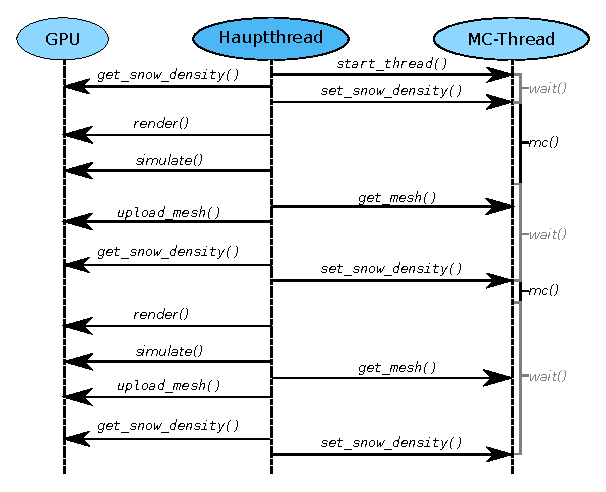
\includegraphics[width=12cm]{images/producer_consumer}
\caption{Das Producer-Consumer-Problem in der Anwendung. Der MC-Thread wartet solange, bis der Hauptthread ihm Daten zur Verfügung stellt. Er verarbeitet die Daten und wartet dann weiter. Der Hauptthread prüft nur an bestimmten Synchronisationspunkten, ob der MC-Thread Daten geliefert hat.}
\label{fig:implementation_fallen_snow_producer_consumer}
\end{figure}

\section{Andere Visualisierungsmöglichkeiten}

\begin{itemize}
\item Rauch
\end{itemize}
